\section{Implementation}
\label{sec:impl}

Section~\ref{sec:design} says when each packet should leave, but a forwarding pipeline has no way
to wait: a P4 program runs to completion per packet and can read a clock, yet it cannot sleep or
schedule a callback.

\subsection{Holding a packet with queues}
\label{sec:impl:queues}

\begin{figure}[t]
\centering
\IfFileExists{figures/fig_design.pdf}{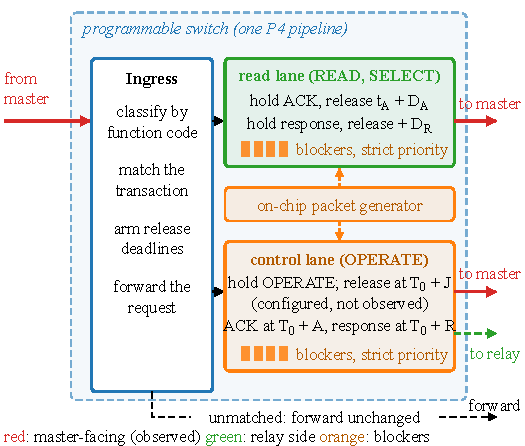
\includegraphics{figures/fig_design}}{\figplaceholder{One P4 pipeline: ingress classifies and arms deadlines; a read lane holds the acknowledgment and the response; a control lane holds the OPERATE; blocker reservoirs drained by a strict-priority scheduler realize the deadlines; unmatched traffic is forwarded.}}
\caption{How one pipeline realizes the schedule. Ingress classifies each transaction and computes
  its release deadlines. Blocker packets drained ahead of the held packet sustain a hold until its
  deadline expires. The four-queue ladder holds what the outstation returns; the second pair holds
  the outgoing OPERATE, not a second reply. Solid lines are master-facing and observed; dashed
  lines are not, as in Figure~\ref{fig:observation}.}
\label{fig:design}
\end{figure}

What the switch does have is a traffic manager with several queues per port and a strict-priority
scheduler, the primitive with which SP-PIFO approximates programmable scheduling on today's
hardware~\cite{alcozSPPIFOApproximatingPushIn2020}. A scheduler decides what does \emph{not}
leave, and we hold a packet by using that property rather than a timer.

A READ uses \emph{four} queues on one internal port, as Figure~\ref{fig:design} shows. Two carry
the packets we delay, the acknowledgment and the response, and above each of those sits a
\emph{blocker queue} in strict priority carrying small packets the switch generates itself. While
blockers keep arriving, the packet beneath them is never served, and each hold ends when its own
blocker queue runs dry. The response is not simply queued behind the acknowledgment: it has its
own held queue and its own blocker gate, which is what lets the two releases be scheduled
independently. In descending priority the ladder is acknowledgment blockers, held
acknowledgment, response blockers, held response.  Blockers circulate on an internal loopback port and never reach a cable, so neither endpoint
can observe them. Each carries a tag naming its transaction and lane, so a leftover blocker
cannot delay a later transaction.

This is not a timer built from a count. The program stores an absolute release instant when the
acknowledgment arrives, quantized to a 256~ns grid, and each of the 64 recirculating blockers
compares the current timestamp against it: while the difference is negative the blocker is
regenerated, and once it is not, the blocker is dropped. The deadline decides when the packet
leaves, and the blockers only have to keep the queue non-empty until then, so the reservoir is
sized for continuity rather than for duration.

The queue does not empty at the deadline, however. Each blocker tests the deadline on its own
pass, so those still queued when it passes are served once more before the queue runs dry and the
held packet leaves. The release therefore trails the deadline by the time that draining takes, and
each lane drains its own queue, the acknowledgment's above the response's;
Section~\ref{sec:eval:limits} reports what we measured of that interval. The arrangement is what
makes the coupling of Section~\ref{sec:design:model} implementable: the response's release instant
is computed at the acknowledgment, so the hold absorbs whatever the outstation does without the switch measuring it.

\subsection{One READ transaction}
\label{sec:impl:walkthrough}

The request arrives, a table classifies it by function code, and the program forwards it at once,
recording that a transaction is in flight and which acknowledgment to expect. When the
acknowledgment arrives at $t_A$, a median of 0.56~ms after the request on our relay, the
program writes both release instants from that one timestamp, which is what puts them on the
same instant $t_A$ that Section~\ref{sec:design:model} requires. It does so once from an unarmed sentinel so a duplicate acknowledgment cannot arm a
second deadline. The acknowledgment enters the hold queue and the packet generator fills the
blocker queue. A response that arrives before its deadline queues behind the acknowledgment,
and the two leave in order at their scheduled instants. A response that arrives after its deadline has no remaining wait to serve, and the program marks
it late and commits it to the same response-hold queue rather than to a bypass, as in
Figure~\ref{fig:timeline}(b); it leaves when that queue next serves it, so its departure is
prompt but not instantaneous. The transaction state is cleared when the response is released.

The two lanes hold different packets, and it is worth saying which. The four-queue ladder above
holds what the outstation sends back, the acknowledgment and the response, for READ and for both
phases of a control alike. The second loopback port carries a pair of queues for the opposite
direction: blockers above a held \emph{OPERATE request}, on its way to the relay. So the control
extension adds a hold the read path does not have, while the packets the master observes are
released by the same machinery in both cases. Giving the OPERATE its own scheduling domain keeps
it from being starved by the higher-priority read reservoirs.

The queues are separate; the transaction state is not. The deadline registers are shared. Every register that
records a transaction holds a single slot, and the control path writes the same release instants
at OPERATE admission that the read path uses, so the program protects one transaction at a time
rather than one per flow.

The evaluated configuration satisfies that assumption by construction: the driver serialises its
exchanges and every capture carries one connection. Where a second transaction would arm while one
is live, the program does not interleave them silently; the arming attempt is classified as busy
and the packet is forwarded unprotected rather than taking the deadline already in progress. That
is a statement about the deadline, not about the rest of the transaction's state: the expected
relay sequence and acknowledgment are written earlier in the same pass than the busy verdict is
reached, so we claim it for the serialized workload we evaluated and not in general. Per-flow
protection would need per-flow state and a way to index it, which this program does not have and
we did not evaluate.

\subsection{Failing open}
\label{sec:impl:failopen}

Almost every path through the program ends in a forwarding decision. A packet outside the protected
session, an unrecognized request, an acknowledgment with no armed transaction and a response whose
transaction has retired are all forwarded unchanged, so such an exchange loses its protection and
still arrives. One path is not like that, and we state it here rather than in the evaluation: the
control lane keeps a released OPERATE's application generation as a spent marker until the next
SELECT clears it, and a later OPERATE carrying that generation is dropped. A retransmission the
master sends to repair an OPERATE lost after the switch forwarded it carries exactly that
generation, so the switch discards the packet that would have repaired the loss
(Section~\ref{sec:eval:limits}). Every hold is bounded by a budget on blocker passes: once a reservoir has spent
its budget the packet is released and its state cleared. That budget counts passes rather than
elapsed time, which is why the horizon $H$ of Section~\ref{sec:design:params}, 30.8~ms here, is
what the control plane computes from the budget and an assumed service rate rather than a
wall-clock deadline the data plane keeps. With the timing mode off the same program forwards
everything immediately, which is how we collected the Timing OFF arm.

\subsection{Resources and testbed}
\label{sec:impl:p4}

The program is about 1{,}560 lines of
P4$_{16}$~\cite{bosshartP4ProgrammingProtocolIndependent2014} for the Tofino Native
Architecture, compiled
with the Barefoot SDE 9.13. It occupies all twelve ingress match-action stages of one pipeline and six egress stages, with
112 tables. State is small: one-entry registers reached by stateful ALU actions, one access per packet per
register, which is what the architecture permits. One 25~Gb/s port carries the master and one 1~Gb/s port the relay, and two further ports are
loopbacks carrying no cable: the first carries the four-queue read ladder, the second the control
extension's pair, blockers above a held OPERATE, in its own scheduling domain so the OPERATE
reservoir cannot be starved by the higher-priority read reservoirs. Six queues across two
loopbacks in all.

Every policy quantity is a runtime table entry, so an operator changes policy by writing entries
rather than loading a program. The loaded build realizes the dual-deadline schedule only: its
arming table admits that mode alone, so the acknowledgment-only and response-only limits of the
model are properties of the design and not settings of this build, and configuring them left both
packets unheld with the measured interval the outstation's own.

The control plane, about 890 lines of Python, brings up ports and queues, installs the
packet-generator configuration, and writes the timing parameters and reads them back. What it
refuses is a clamp, not the admission arithmetic: a request for an acknowledgment hold above
40~ms is rejected outright before any write, which we confirmed on the switch, and the
acknowledgment offset $A$ on the control lane must exceed the largest admissible $J$ plus a bound
on the outstation's acknowledgment latency. The horizon $H$ of
Section~\ref{sec:design:params} is computed and reported, not enforced, which is exactly why the
sweep of Section~\ref{sec:eval:policy} can install settings beyond it and find where the
mechanism leaves its operating region. The outstation is an SEL-751A feeder
protection relay, one of the DNP3 device classes whose timing Formby et al.\
fingerprint~\cite{formbyWhosControlYour2016}. The master issues READ and select-before-operate
operations to isolated control points through a guarded driver, so no control operation in the
evaluation moves a breaker.
